\chapter{Literature Review}
\label{chapter:literature-review}

% TODO: Write your literature review here

\section{Introduction}
% Brief overview of what this chapter covers and how it is organized.

\section{Search Strategy}
% Describe how you conducted the literature search.
% Include: databases searched, search strings used, time frame, inclusion/exclusion criteria.
% Reference your SLR protocol if applicable.

\section{Thematic Analysis}
% Organize the literature by themes, not by individual papers.

\section{Theme 1}
% Describe the first main theme emerging from the literature.

\subsection{Subtopic 1.1}

\subsection{Subtopic 1.2}

\section{Theme 2}
% Describe the second main theme.

\subsection{Subtopic 2.1}

\subsection{Subtopic 2.2}

\section{Theme 3}
% Describe the third main theme.

\section{Summary and Research Gap}
% Summarize the key findings from the literature.
% Identify the gap your research addresses.
% Explain how your work contributes to filling this gap.

\section{Chapter Summary}
% Brief recap of the main points covered in this chapter.

% ============================================================
% CITATION EXAMPLES — Remove this section after learning
% ============================================================
% This section demonstrates different citation styles with
% biblatex APA 7th edition. Remove before final submission.

\section*{Citation Examples (Remove Before Submission)}
\addcontentsline{toc}{section}{Citation Examples}

\subsection*{Textual Citations (Author as Subject)}

% Single author
Deep learning has transformed artificial intelligence \textcite{lecun2015deep}.

% Two authors
\textcite{yannakakis2018game} developed a comprehensive framework for AI in games.

% Three or more authors (use ``et al.'')
\textcite{mnih2015atari} achieved human-level control through deep reinforcement learning.

% Multiple citations by same author
\textcite{knuth1997art} described fundamental algorithms in computer science.

\subsection*{Parenthetical Citations (Author in Parentheses)}

% Single citation
Deep learning has transformed artificial intelligence \parencite{lecun2015deep}.

% Multiple citations (alphabetical order)
Several works have explored AI in games \parencite{mnih2015atari, yannakakis2018game}.

% Citation with page number
Shannon's theory remains foundational \parencite[see][pp. 379--383]{shannon1948mathematical}.

% Citation with prefix/suffix
As noted by \textcite[p.~436]{lecun2015deep}, deep learning has achieved remarkable results.

\subsection*{Combining Textual and Parenthetical}

\textcite{colton2012creativity} proposed that computational creativity is the final frontier
\parencite[p.~22]{colton2012creativity}.

\subsection*{Citing Specific Elements}

% Page number
\parencite[p.~45]{pressman2014software}

% Chapter
\parencite[Chapter~3]{knuth1997art}

% Figure/Table
\parencite[Figure~1]{goodfellow2016generative}

% No author (use title)
\parencite{artificial2020intelligence}

% ============================================================
% END CITATION EXAMPLES
% ============================================================

% ============================================================
% TABLE AND FIGURE EXAMPLES — Remove this section after learning
% ============================================================
% This section demonstrates how to create tables and figures.
% Remove before final submission.

\section*{Tables and Figures Examples (Remove Before Submission)}
\addcontentsline{toc}{section}{Tables and Figures Examples}

\subsection*{Simple Table}

\begin{table}[htbp]
    \centering
    \caption{Summary of Research Methods}
    \label{tab:research-methods}
    \begin{tabular}{lll}
        \toprule
        \textbf{Method} & \textbf{Type} & \textbf{Best For} \\
        \midrule
        Survey & Quantitative & Large samples \\
        Interview & Qualitative & In-depth understanding \\
        Experiment & Quantitative & Cause-effect relationships \\
        Case Study & Qualitative & Specific contexts \\
        \bottomrule
    \end{tabular}
\end{table}

As shown in Table~\ref{tab:research-methods}, different methods serve different purposes.

\subsection*{Table with Multiple Columns}

\begin{table}[htbp]
    \centering
    \caption{Comparison of AI Approaches}
    \label{tab:ai-comparison}
    \begin{tabular}{p{3cm}p{4cm}p{4cm}}
        \toprule
        \textbf{Approach} & \textbf{Advantages} & \textbf{Disadvantages} \\
        \midrule
        Supervised Learning & High accuracy with labeled data & Requires large labeled datasets \\
        Unsupervised Learning & No labels needed & Harder to evaluate \\
        Reinforcement Learning & Solves complex problems & Training can be unstable \\
        \bottomrule
    \end{tabular}
\end{table}

\subsection*{Figure (Placeholder)}

% To include an image, use:
% \begin{figure}[htbp]
%     \centering
%     \includegraphics[width=0.8\textwidth]{figures/your-image.png}
%     \caption{Description of the figure}
%     \label{fig:your-figure}
% \end{figure}
%
% Reference it in text: Figure~\ref{fig:your-figure}

\subsection*{Figure with Subfigures}

\begin{figure}[htbp]
    \centering
    \begin{subfigure}{0.45\textwidth}
        \centering
        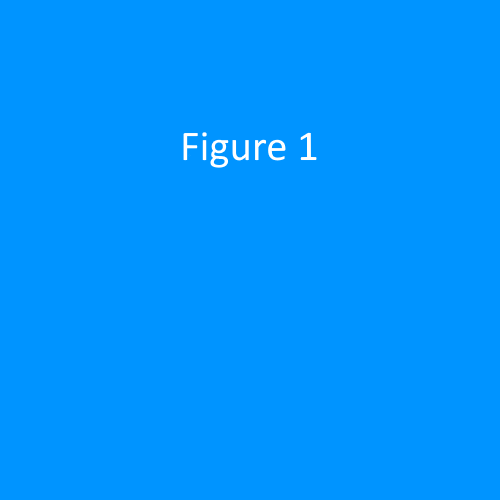
\includegraphics[width=\textwidth]{figures/image1.png}
        \caption{First subfigure}
        \label{fig:sub1}
    \end{subfigure}
    \hfill
    \begin{subfigure}{0.45\textwidth}
        \centering
        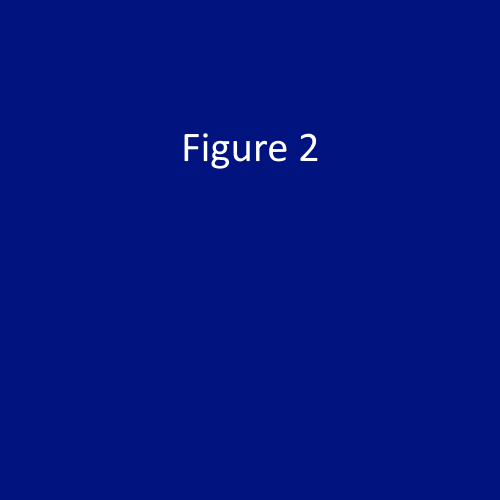
\includegraphics[width=\textwidth]{figures/image2.png}
        \caption{Second subfigure}
        \label{fig:sub2}
    \end{subfigure}
    \caption{Comparison of two approaches}
    \label{fig:comparison}
\end{figure}

Reference in text: Figure~\ref{fig:sub1} and Figure~\ref{fig:sub2}

\subsection*{Algorithm}

% To include an algorithm, use:
% \begin{algorithm}[htbp]
%     \caption{Example Algorithm}
%     \label{alg:example}
%     \begin{algorithmic}[1]
%         \State \textbf{Input:} Data $X$
%         \State \textbf{Output:} Result $Y$
%         \For{each $x$ in $X$}
%             \State Process $x$
%         \EndFor
%         \State \textbf{return} $Y$
%     \end{algorithmic}
% \end{algorithm}

% ============================================================
% END TABLE AND FIGURE EXAMPLES
% ============================================================
